%-----------------------------------------------
% Template para criação de resumos de projectos/dissertação
% jlopes AT fe.up.pt,   Fri Jul  3 11:08:59 2009
%-----------------------------------------------

\documentclass[9pt,a4paper]{extarticle}

%% English version: comment first, uncomment second
\usepackage[portuguese]{babel}  % Portuguese
%\usepackage[english]{babel}     % English
\usepackage{graphicx}           % images .png or .pdf w/ pdflatex OR .eps w/ latex
\usepackage{times}              % use Times type-1 fonts
\usepackage[utf8]{inputenc}     % 8 bits using UTF-8
\usepackage{url}                % URLs
\usepackage{multicol}           % twocolumn, etc
\usepackage{float}              % improve figures & tables floating
\usepackage[tableposition=top]{caption} % captions
%% English version: comment first (maybe)
\usepackage{indentfirst}        % portuguese standard for paragraphs
%\usepackage{parskip}

%% page layout
\usepackage[a4paper,margin=30mm,noheadfoot]{geometry}

%% space between columns
\columnsep 12mm

%% headers & footers
\pagestyle{empty}

%% figure & table caption
\captionsetup{figurename=Fig.,tablename=Tab.,labelsep=endash,font=bf,skip=.5\baselineskip}

%% heading
\makeatletter
\renewcommand*{\@seccntformat}[1]{%
  \csname the#1\endcsname.\quad
}
\makeatother

%% avoid widows and orphans
\clubpenalty=300
\widowpenalty=300

\begin{document}

\title{\vspace*{-8mm}\textbf{\textsc{Electronic Assessment for Software Development Certifications}}}
\author{\emph{Nelson Daniel Ribeiro Mendes}\\[2mm]
\small{Dissertation held under the guidance of \emph{Prof.\ João Pascoal Faria}}\\
\small{at \emph{Strongstep - Innovation In Software Quality, Lda}}}
\date{}
\maketitle
%no page number 
\thispagestyle{empty}

\vspace*{-4mm}\noindent\rule{\textwidth}{0.4pt}\vspace*{4mm}

\begin{multicols}{2}

\section{Motivation}\label{sec:motiva}

Due to the change of the paradigm of current markets, resulting from the phenomenon of globalization, organizations are forced to streamline their business, in order to be able to maintain their competitiveness and ensure a favorable market position. To achieve such agility, their processes need to be less time consuming and more effortless, so they can focus on what really matters: value creation.

Certifications are a formal recognition of an organization that will provide guidance and tools for those who want to ensure that their products and services consistently meet customer's requirements, and that quality is consistently improved. However useful for the organization, the evaluation for certification takes too much effort and time. For example, the SCAMPI method takes a significant effort, being in some cases a very painful and expensive process. SCAMPI is the Standard CMMI Appraisal Method for Process Improvement, the evaluation method of CMMI model. CMMI is a model for organizations to improve their processes and is required by many U.S. Government contracts, especially in software development. 



\section{Objectives}\label{sec:goals}
Tool support is fundamental for facilitating the adoption of CMMI practices. SCRAIM \cite{SCRAIM} is an example of a project life cycle management tool specifically designed to facilitate CMMI implementations.
The main goal is of this dissertation is to develop a group of methodologies, techniques and tools integrated in the SCRAIM, that will make evaluations and certain parts of certifications easier and less painful for the SCRAIM users.

More specifically, the goals of this dissertation work are as follows:

\begin{itemize}%for capital roman numbers.
	\item Analyze to what extent the SCRAIM tool supports the implementation (including the collection of evidences) of the specific practices of CMMI-DEV \cite{Development2010} for maturiy levels 2 and 3 (ML2-3), and recommend relevant improvements to SCRAIM;
	\item Define rules to automatically assess the degree of fulfillment of CMMI-DEV ML2 practices by SCRAIM users, by analysing organizational project data and any other relevant evidences recorded in SCRAIM;
	\item Define questionnaires to assist the users in doing a manual assessment, for the practices  of CMMI-DEV ML2 that cannot be assessed automatically, ;
	\item Implement in SCRAIM rules and questionnaires defined in steps (ii) and (iii), for some process areas, including appropriate user interfaces to conduct assessments and visualize assessment results;
	\item Validate the electronic assessment approach in real world projects.
\end{itemize}


\section{Work description}\label{sec:work}

\subsection{State of the art}

Several electronic assessment tools are currently being used in order to assist appraisers in their field work. Other tools allow the user to obtain a rating based on their responses.

Were studied the following tools:
\begin{itemize}
	\item CMMI assessment checklist \cite{capabilityassess}
	\item PSPchecker \cite{Pinto2010}
	\item Appraisal assistant \cite{Appraisal2015}
	\item ITMark appraisal tool ~\cite{ITMARKASSESSMENT}
\end{itemize}


\subsection{Conception}
One of the objectives of this thesis was to understand the level of support of SCRAIM in the CMMI scenario; this is researched and presented in the dissertation, making an assessment of SCRAIM with the help of another tool that is currently used by appraisers.

Was created a process in order to achieve the electronic assessment and handling the automatic part (rule based) and the manual part (question based). Those rules and questionnaires were conceived to enable semi-automatic SCAMPI evaluations.
The questions were selected for the questions that could not be evaluated with the rules.

Some of the gaps found could be solved be solved with the integration of some plugins, frameworks and rules of usage, and are presented too those recommendations.

\subsection{Implementation}

After defining the rules was necessary to validate them, for that an implementation of those the rules was mandatory.

The prototype developed was implemented on top of SCRAIM and the architecture was another point of work, in order to get a flexible and scalable architecture, taking for base the same technologies that it uses.
An  expansion of the database was done, inserting new tables and an adding models, views and controls to Ruby on Rails in order to implement this prototype on top of SCRAIM. All expansions can be seen in  Figure \ref{fig:figura}.

\begin{figure}[H]
	\centerline{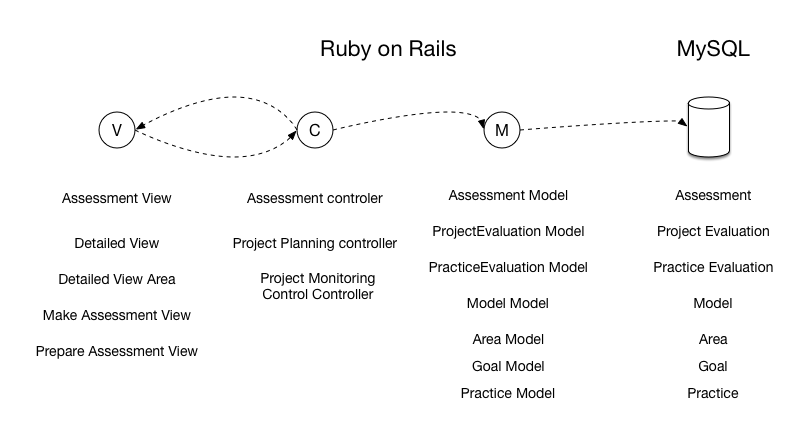
\includegraphics[scale=.3]{presentation.png}}
	\caption{Data Model of the tables added to the SCRAIM database}  
	\label{fig:figura}
\end{figure}



\subsection{Results}

To determine if the electronic assessment generates results close to a manual assessment performed by an expert it is necessary to compare an automatic assessment (performed by the tool) to a manual assessment (performed by a human expert).

In both assessments only the two areas featured in the current implementation of this module are considered for comparison.

The distribution of the difference and matching of the two results are shown in Figure \ref{fig:figura2}.

\begin{figure}[H]
	\centerline{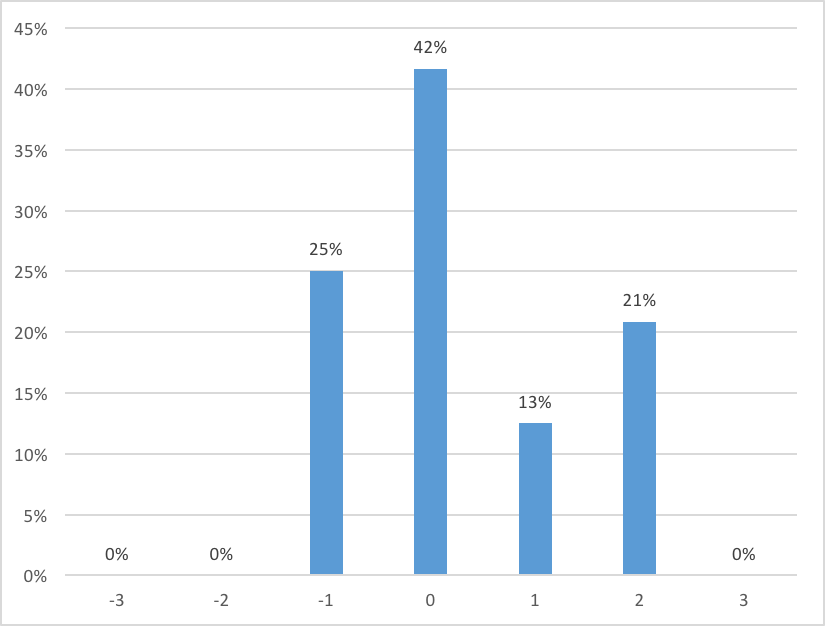
\includegraphics[scale=.5]{delta.png}}
	\caption{Distribution of electronic assessment errors}  
	\label{fig:figura2}
\end{figure}


It is possible to see that the electronic automatic ratings that differ by 2 from the manual assessment are still 21\%. The explanation for the difference is that actually it is impossible to check the content of documents submitted to SCRAIM; in some cases just for using SCRAIM  it is automatically considered the last level or some practices are evaluated in only two levels, the maximum level (4) or the minimum level (1) . For example the practice PP.SP1.1 is rated differently because in the automatic assessment is only seen if WBS are defined and epics are associated with backlog items, but in the manual assessment it is seen the preliminary report submitted on SCRAIM that contains some evidences for this practice not possible to evaluate yet
automatically.

\subsection{Conclusions}
All the goals established in the start of this thesis were almost completely fulfilled. The group of tools, methodologies and techniques accomplished resulted in a prototype of an automatic assessment module in SCRAIM. The results generated by the prototype are promising, getting very close to a real assessment.
It was intended to reduce the costs and time of a SCAMPI evaluation and with the comparative analysis made we can say that this approach will make that happen and the prototype when extended and completed with the future work will facilitate the SCAMPI appraisals.


%%English version: comment first, uncomment second
%\bibliographystyle{unsrt-pt}  % numeric, unsorted refs
\bibliographystyle{unsrt}  % numeric, unsorted refs
\bibliography{refs}

\end{multicols}

\end{document}
